\section{Primary results and inference}
\label{sec:results}

\subsection{Realized performance}

Table~\ref{tab:table1_performance} reports the six strategies over
2010--2026, net of 10 basis points. The regime-aware strategy earned a
Sharpe ratio of \regimeSharpe{} against the comparator's
\comparatorSharpe{}. Reading down the ladder, most of the risk-adjusted
gain over the naive benchmarks comes from optimization itself rather
than from anything dynamic: equal weight earns \equalWeightSharpe{} and
static minimum variance \staticMinvarSharpe{}, after which dynamic
covariance adds nothing measurable (\comparatorSharpe{}) and the two
responsive rungs add modest further amounts.

The highest realized Sharpe in the ladder belongs to the
volatility-scaled strategy (\ewmaScaledSharpe{}), not to the regime-aware strategy.
That was not predicted by the design and is reported as found; it does
not alter the preregistered hypothesis, which concerns the regime rung.

\begin{table}[htbp]
\caption{Realized performance, 2010--2026, net of 10 basis points. Annualized figures; maximum drawdown from the net wealth path.}
\label{tab:table1_performance}
\small
\begin{tabular}{lrrrrrr}
\toprule
 & CAGR (\%) & Volatility (\%) & Sharpe & Sortino & Max DD (\%) & Calmar \\
\midrule
Equal weight & 11.61 & 11.90 & 0.857 & 1.214 & $-$22.80 & 0.509 \\
60/40 & 9.82 & 9.78 & 0.852 & 1.207 & $-$21.20 & 0.463 \\
Static min-var & 9.04 & 8.23 & 0.910 & 1.301 & $-$19.17 & 0.471 \\
Rolling LW min-var & 8.71 & 7.88 & 0.908 & 1.293 & $-$17.41 & 0.500 \\
EWMA-scaled min-var & 8.70 & 7.54 & 0.945 & 1.356 & $-$17.30 & 0.503 \\
Regime-aware min-var & 8.73 & 7.71 & 0.929 & 1.331 & $-$17.44 & 0.501 \\
\bottomrule
\end{tabular}
\end{table}


\subsection{The preregistered comparison}

The estimated difference in annualized net Sharpe ratio between the
regime-aware strategy and rolling Ledoit--Wolf minimum variance is
\begin{equation}
\widehat{\Delta SR} = \primarySharpeDiff, \qquad
\text{95\% CI } [\primaryCiLower,\ \primaryCiUpper], \qquad
p = \primaryPValue .
\end{equation}

The interval is roughly \ciWidthMultiple{} times as wide as the point
estimate and contains zero comfortably; the estimate sits
\primarySdsFromZero{} bootstrap standard deviations from zero. $H_0$ is
not rejected.

Inference uses a stationary bootstrap with 10{,}000 replications, mean
block length 21 trading days and seed 12345, applied to \emph{paired
daily excess returns} annualized by $\sqrt{252}$ --- the same estimand
the point estimate reports. Both strategies receive identical bootstrap
indices in every replication, preserving contemporaneous pairing; a test
confirms that feeding the same series twice yields exactly zero
difference with zero variance. The one-sided $p$-value comes from the
centered null $\Delta SR_b - \widehat{\Delta SR}$, not from the fraction
of ordinary draws below zero, which is a different quantity.

The conclusion is insensitive to block length: mean blocks of 10, 42 and
63 days all produce interval bounds within \blockMaxDeviation{} of the
primary bounds, and every one contains zero.

\subsection{Returns and volatility separately}

Mean returns are indistinguishable. Paired daily net return differences
give an annualized arithmetic difference of \hacAnnualReturnDiff{}
against a Newey--West standard error of \hacStandardError{}, so the
estimate sits \hacSdsFromZero{} standard errors from zero
($p = \hacPValue{}$, HAC lag 21; lags of 5 and 42 give the same
conclusion).

Among the \nSecondaryMetrics{} secondary metric intervals, only
annualized volatility excludes zero: the regime-aware strategy's is
lower by \volDifferenceMagnitude{}, with a 95\% interval on that
difference running from \volCiLower{} to \volCiUpper{}. This is a secondary, unadjusted interval among several examined
metrics and is not confirmatory evidence. What raises it above an
incidental finding is that it is the outcome the mechanism predicts: a
variance minimizer given additional information about variance should
reduce variance. It is not described as statistically established.

\subsection{Trading costs}

The regime-aware strategy trades \regimeHalfTurnover{} annual
half-turnover against the comparator's \comparatorHalfTurnover{}, a
factor of \turnoverRatio{}. At the primary cost assumption it spends
\regimeCost{} per year against the comparator's \comparatorCost{}, a
hurdle of \costHurdle{} that its risk reduction must clear. The estimated
Sharpe advantage falls monotonically with costs, from \diffAtZeroBps{} at
zero to \diffAtTwentyBps{} at 20 basis points, and no cost level produces
an interval excluding zero.

\begin{table}[htbp]
\caption{Preregistered primary comparison. Paired stationary bootstrap, 10{,}000 replications, mean block 21 trading days, seed 12345, on daily excess returns.}
\label{tab:table2_primary_inference}
\small
\begin{tabular}{lrrrr}
\toprule
 & $\Delta$ Sharpe & CI lower & CI upper & p-value \\
\midrule
Regime-aware $-$ rolling LW & 0.021 & $-$0.075 & 0.115 & 0.327 \\
\bottomrule
\end{tabular}
\end{table}


\section{Robustness}
\label{sec:robustness}

Thirteen specifications each vary one factor at a time from the primary
model; no Cartesian product is constructed. Figure~\ref{fig:forest}
shows the Sharpe difference and its interval across all of them, ordered
as declared before any result was seen rather than sorted by effect.

\begin{figure}[htbp]
\centering
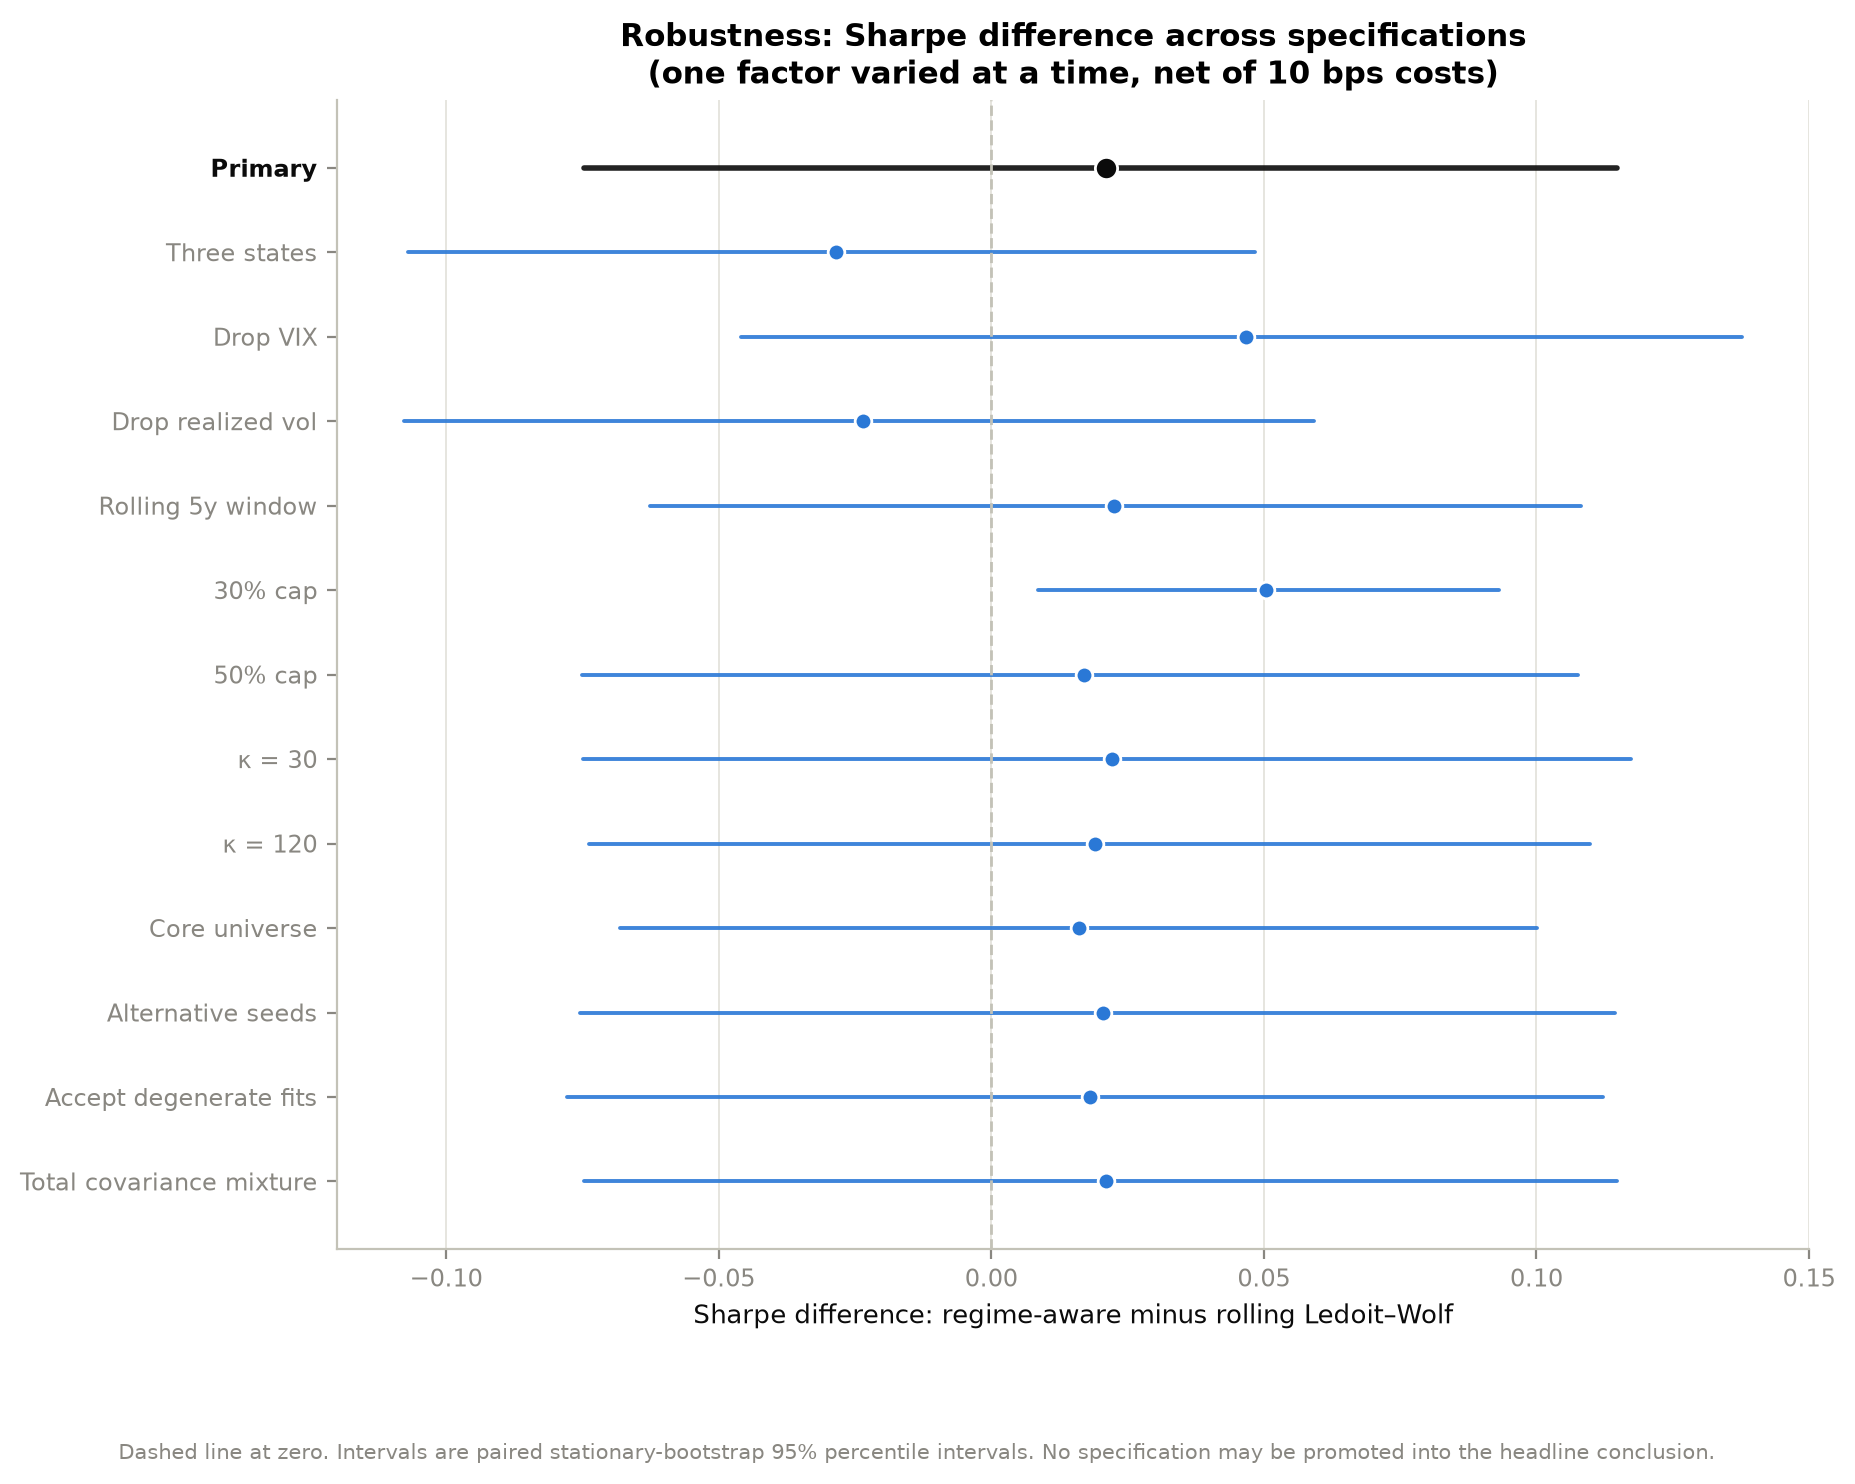
\includegraphics[width=\textwidth]{figures/robustness_forest.png}
\caption{Sharpe difference between the regime-aware strategy and rolling
Ledoit--Wolf minimum variance across thirteen specifications, each
varying one factor. Intervals are paired stationary-bootstrap 95\%
percentile intervals; the primary specification is shown in black. Only
the 30\% weight cap excludes zero, and it does not survive Holm
adjustment.}
\label{fig:forest}
\end{figure}

Point estimates are positive in \nSpecsPositive{} of the thirteen
specifications, and \nSpecsContainingZero{} of the thirteen intervals
contain zero. \textbf{After Holm adjustment across the
twelve-specification robustness family, nothing survives.}

\paragraph{Sign instability.} The estimate reverses sign in
\nSignReversals{} of the preregistered variations: the three-state HMM
(\threeStateDiff{}) and dropping realized
volatility from the feature set (\dropRvDiff{}). Neither reversal is
significant, but a result that changes direction when the state count
changes is fragile. The three-state model is not itself defective --- its
middle state holds \threeStateMidOccupancy{} occupancy with a minimum
effective sample size of \threeStateMinNeff{}, canonical
low--medium--high ordering holds at every refit, and no initialization
failed --- so the reversal reflects the estimate rather than a broken
fit.

\paragraph{The weight cap.} The 30\% cap is the only specification whose
unadjusted interval excludes zero (\capThirtyDiff{},
$p = \capThirtyP{}$), and it does not survive Holm adjustment
($p = \capThirtyPHolm{}$). Decomposing it exactly, using
$\Delta SR(\text{0 bps}) - \Delta SR(\text{10 bps})$ rather than
approximating cost expenditure divided by volatility: reduced cost drag
accounts for \capThirtyCostComponent{} of the \capThirtyTotalChange{}
change from the 40\% cap (\capThirtyCostShare{}), while gross pre-cost
differences account for \capThirtyGrossComponent{}
(\capThirtyGrossShare{}). Under the 30\% cap the volatility advantage disappears while
the relative turnover penalty falls substantially; however, reduced
transaction costs explain only part of the larger Sharpe difference,
with altered portfolio exposures and gross-return realizations
accounting for the remainder.

\paragraph{Factors that barely move the estimate.} The complete
total-covariance mixture reproduces the primary estimate to four
decimals, confirming the measured negligibility of the omitted
between-state term. Shrinkage thresholds of 30 and 120 move the estimate
by at most \kappaMaxMove{}. An alternative seed block gives
\altSeedsDiff{} against the primary \primarySharpeDiff{}, despite the
selected seed changing at \refitSeedChanges{} of 199 consecutive refits.
Accepting the degenerate fits rather than falling back gives
\aTwoAcceptDiff{}.

\paragraph{Subperiods.} Sliced descriptively from the primary paths, the
pre-2020 estimate is \preTwentyTwentyDiff{} and the post-2020 estimate is
\postTwentyTwentyDiff{}. With \covidDays{} days in the COVID slice and
\tighteningDays{} in the 2022 tightening slice,
these samples are far too small for inference, and the sign disagreement
between halves of the sample is a further reason for caution about the
full-sample point estimate. No subperiod is promoted.

\begin{table}[htbp]
\caption{Robustness grid: thirteen specifications, each varying one factor from the primary model.}
\label{tab:table4_robustness_grid}
\small
\begin{tabular}{lrrrr}
\toprule
 & $\Delta$ Sharpe & CI lower & CI upper & $\Delta$ Vol (pp) \\
\midrule
Primary & 0.021 & $-$0.075 & 0.115 & $-$0.175 \\
Three states & $-$0.028 & $-$0.107 & 0.048 & $-$0.180 \\
Drop VIX & 0.047 & $-$0.046 & 0.138 & $-$0.117 \\
Drop realized vol & $-$0.023 & $-$0.108 & 0.059 & $-$0.052 \\
Rolling 5y window & 0.022 & $-$0.063 & 0.108 & $-$0.206 \\
30\% cap & 0.050 & 0.009 & 0.093 & 0.033 \\
50\% cap & 0.017 & $-$0.075 & 0.108 & $-$0.137 \\
$\kappa$ = 30 & 0.022 & $-$0.075 & 0.117 & $-$0.175 \\
$\kappa$ = 120 & 0.019 & $-$0.074 & 0.110 & $-$0.177 \\
Core universe & 0.016 & $-$0.068 & 0.100 & $-$0.188 \\
Alternative seeds & 0.020 & $-$0.075 & 0.114 & $-$0.175 \\
Accept degenerate fits & 0.018 & $-$0.078 & 0.112 & $-$0.171 \\
Total covariance mixture & 0.021 & $-$0.075 & 0.115 & $-$0.175 \\
\bottomrule
\end{tabular}
\end{table}


\section{Limitations}
\label{sec:limitations}

\paragraph{Precision.} Despite approximately \oosYears{} years of out-of-sample
returns, the study had limited precision for detecting small differences
in risk-adjusted performance. The estimated Sharpe difference was
\primarySharpeDiff{}, while its 95\% bootstrap interval ranged from
\primaryCiLower{} to \primaryCiUpper{}. Consequently, the analysis
provides no confirmatory evidence of improvement, but it also cannot
exclude economically modest positive or negative effects. The results
should therefore be interpreted as inconclusive regarding small effects
rather than as evidence that regime conditioning has exactly zero value.

The binding constraint is information rather than raw observation count.
Inference uses daily paired returns, but the strategy makes only about
200 rebalancing decisions, and serial dependence in both returns and
regime states further reduces the effective information available to
distinguish two highly correlated strategies.

\paragraph{Universe selection.} Exchange-traded funds avoid single-name
survivorship bias, but choosing these five funds in 2026 uses knowledge
that they survived and remained liquid. All conclusions are conditional
on the universe.

\paragraph{Vendor data.} Yahoo adjusted closes are restated when
distributions occur, so the analysis is tied to a specific frozen
snapshot rather than to a canonical dataset. Cross-validation against
CRSP or a commercial vendor would strengthen it.

\paragraph{Cost model.} Costs are proportional to traded notional. The
model excludes market impact, taxes, borrowing constraints and bid--ask
dynamics, all of which would penalize the higher-turnover strategies
further.

\paragraph{Scope.} One market, one asset-class mix, one regime
specification family. Whether the finding extends to international
assets, credit, or intraday-informed volatility estimates is untested.

\paragraph{Numerical reproduction.} Two independent runs produced
filtered probabilities differing by up to \reproductionMaxDifference{},
while all selected seeds, classifications and reported conclusions
reproduced. Exact argmax selection and tolerance-based selection were
each stable across the two runs, although they selected different seeds
at \argmaxToleranceDisagreements{} of
200 origins. The evidence therefore supports numerical stability of both
rules but does not establish that the tolerance rule was necessary for
reproduction.

\paragraph{Researcher discretion.} Preregistration, frozen data, causal
tests, automated validation and dated amendments substantially
constrained ex-post researcher discretion. All amendments were
documented before viewing the results they could influence. Discretion
was constrained, not eliminated: implementation choices were made
throughout, and four amendments modified the frozen plan after it was
tagged.
